\section{Active Global Address Space}
\label{agas}

This section provides an overview of the implementation of the Active Global
Address Space (AGAS) in HPX runtime system.

AGAS is a global memory addressing system that is designed to
handle various memory configurations ranging from those implemented in single small
machines to those typically found in a cluster composed of a large number of
nodes with heterogeneous computing resources. AGAS is designed such that
specific memory configuration characteristics are handled by the programmer
through the API. Fig.
\ref{fig:agas_struct} illustrates AGAS's role in HPX. Typically, 
each part of the distributed AGAS service is hosted on a separate node of a
cluster. AGAS consists of several subsystems that are depicted in Fig.
\ref{fig:agas_intern} and are the following:

\begin{figure}[t]
    \centering
    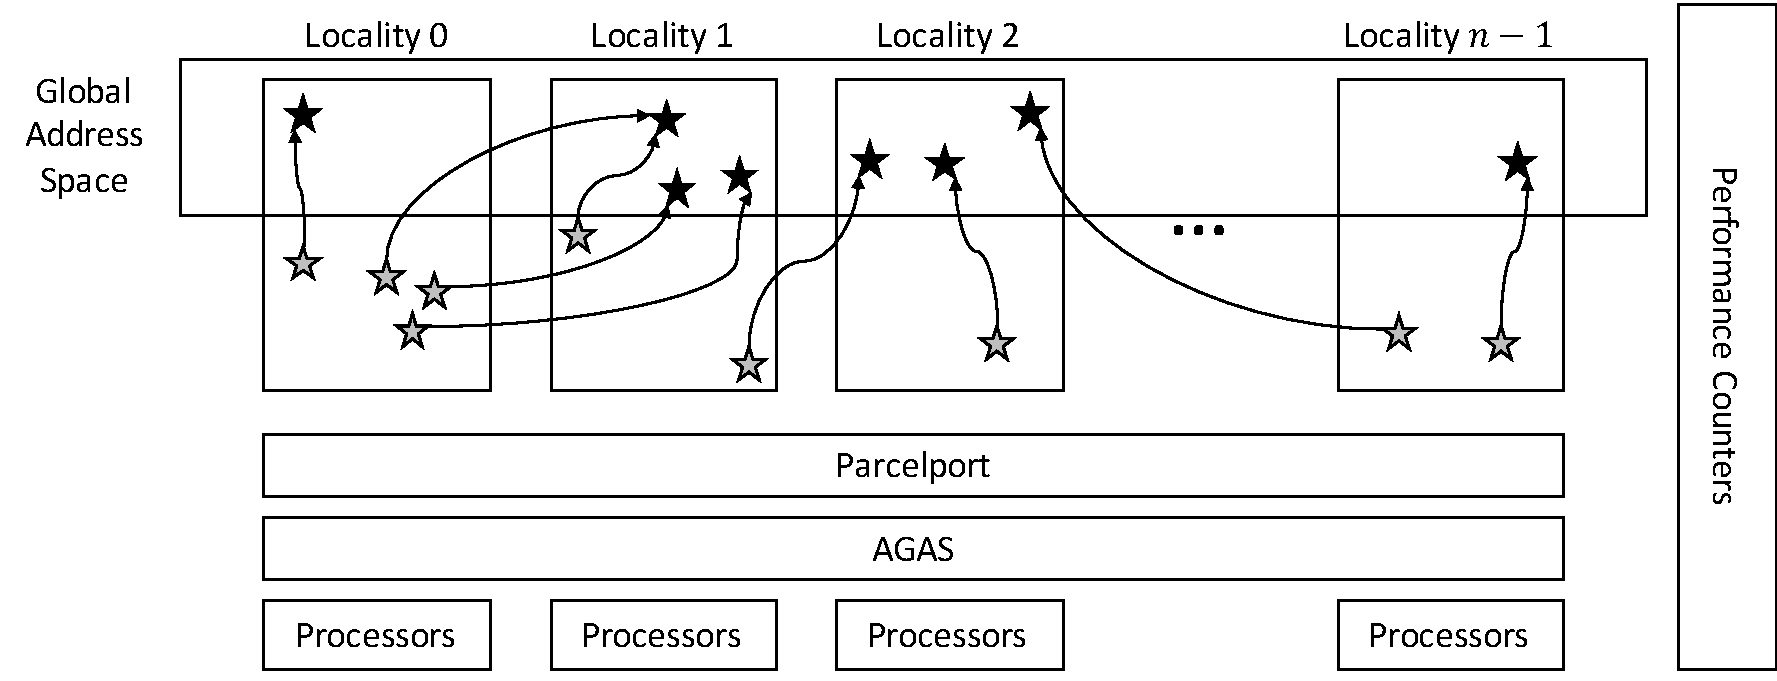
\includegraphics[width=.49\textwidth,height=\textheight,keepaspectratio]{illustrations/agas_struct}
    \caption{AGAS provides an abstraction layer on top of virtual addresses local to each locality. Global objects are shown as black stars and gray stars indicate references to global objects. Each reference is connected to global objects by an arrow.}
    \label{fig:agas_struct}
\end{figure}
\begin{figure}[t]
    \centering
    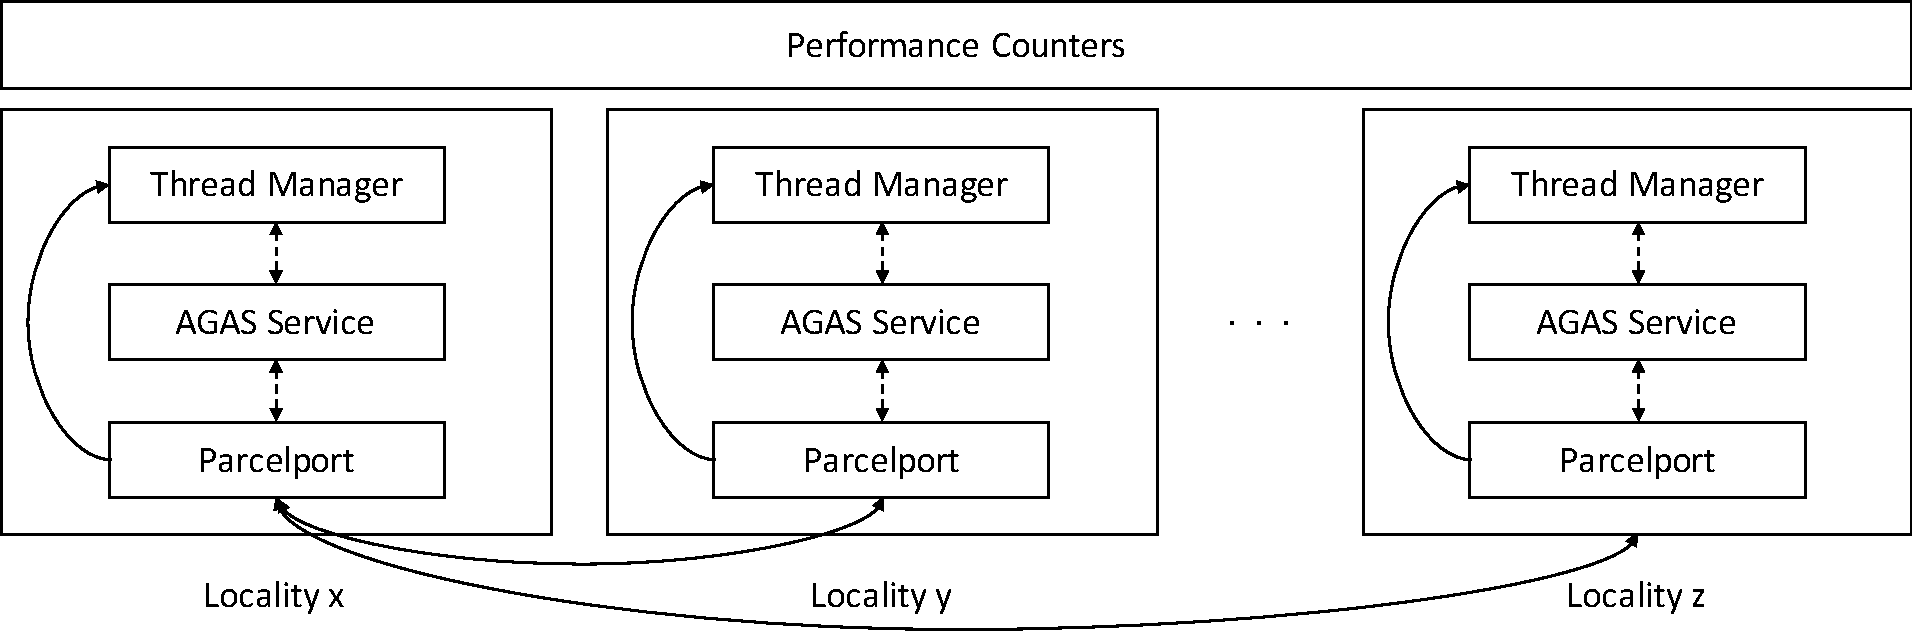
\includegraphics[width=.49\textwidth,height=\textheight,keepaspectratio]{illustrations/agas_interaction}
    \caption{When an HPX thread accesses a global object, AGAS determines if the object can be accessed locally. If the object is on a different locality the HPX thread is serialized and given to the parcelport. The parcelport unserializes the task and hands it to the thread manager for execution.}
    \label{fig:agas_interaction}
\end{figure}

%\begin{figure*}[t!]
%    \centering
%    \begin{subfigure}[t]{.5/\textwidth}
%        \centering
%        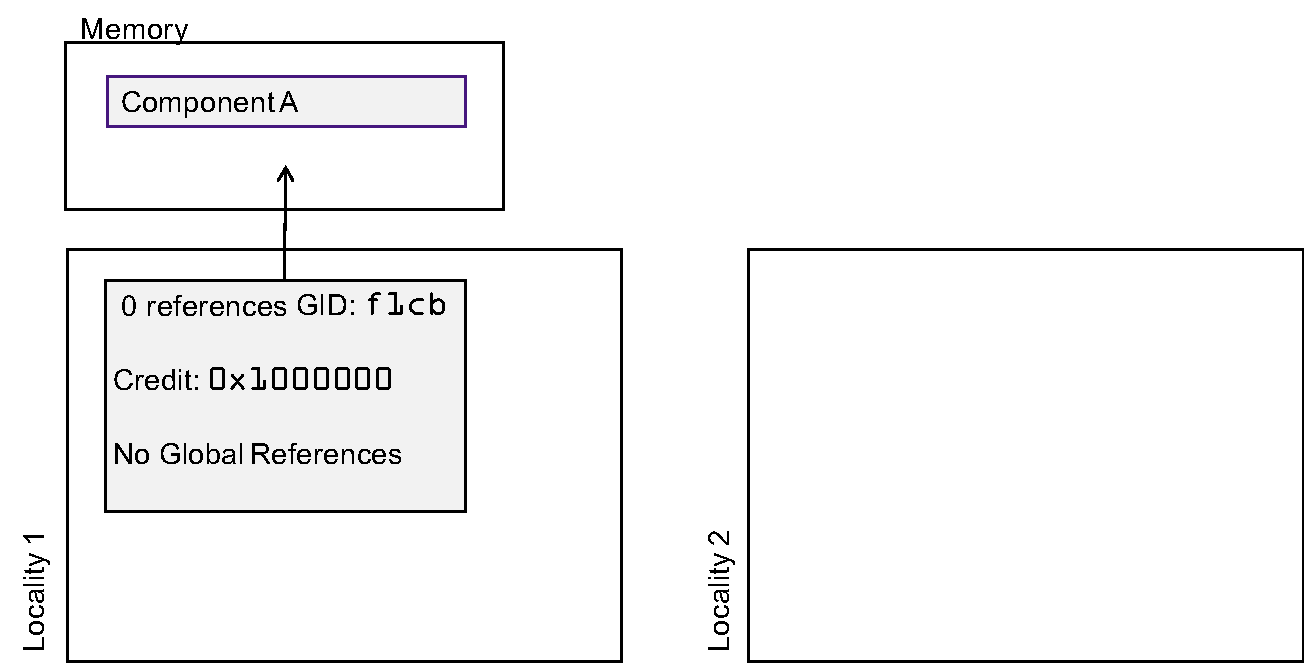
\includegraphics[width=.49\textwidth,height=\textheight,keepaspectratio]{illustrations/reference_counting_1}
%        \caption{}
%    \end{subfigure}
%    \label{fig:agas_ref_count_1}
%\end{figure*}

\begin{enumerate}
    \item{Primary Namespace:
        To provide uniform access to objects across the boundaries
        of physical partitions in a cluster, AGAS provides applications
        with 128-bit global identifiers (GIDs) to be used in place of
        virtual addresses that are local to specific nodes.
        Consequently, AGAS maintains mapping tables to be able to map GIDs
        to local virtual addresses.}
    \item{Locality Namespace:
        Information about the nodes and computing resources allocated to
        each physical partition is held in the locality namespace. Each 
        partition is called a "locality" and locality 0 is responsible for 
        maintaining current information about all other localities.}
    \item{Component Namespace:
        Types are registered in this namespace to facilitate resolving resource 
        requirements during bulk memory allocations.}
    \item{Symbolic Namespace:
		The symbolic namespace is a layer on top of the global address space
		that allows mapping symbolic names to global addresses for the purpose
		of resolving global addresses at runtime. This is useful in cases where
		data about specific events needs to be collected. For example, HPX
		performance counter system uses the symbolic namespace for collecting
		performance counter data.}
    \item{AGAS Cache:
		AGAS cache stores mapping between the most recently used global
		addresses to localities where those object reside and local virtual addresses. If a task requires
		an object that does not live on the same locality then the task is sent
		to the locality where the object currently is. However, in order to do
		so, AGAS has to determine the current location of the queried object.
		If AGAS does not know the current location then it forwards the query
		to the locality where the object was originally created. The locality
		on which an object is created stays responsible for maintaining the
		current location of the object during its entire lifetime. If an object
		is likely to be accessed again then the locality that forwards a task
		will also request the original locality to report the object's current
		location. This information is stored in the AGAS cache. The AGAS cache
		is small since it is designed for speed and therefore, it does not know
		all local objects.}
    \item{Garbage Collection:
        A distributed garbage collection system tracks objects during their
        lifetime and frees the consumed memory when an object goes out of
        scope and therefore can no longer be accessed in the program. HPX
        complies to the C++ standard specifications and hence, it provides
        structures similar to what the modern C++ standard requires.
        Additionally, GIDs in HPX can be managed or unmanaged and in case of
        the former AGAS tracks that GID until the reference is lost so that it
        can free up the memory space when possible. AGAS uses reference
        counting to determine if there are existing references to an object and
        a credit-based scheme for remote references. The local counter is
        updated when a new reference is created and when a reference goes out
        of scope on the same locality. As for remote references, the credit
        system works as demonstrated in Fig. \ref{fig:agas_credit}}

        \begin{figure*}[t]
            \centering
            \begin{subfigure}[t]{0.49\textwidth}
                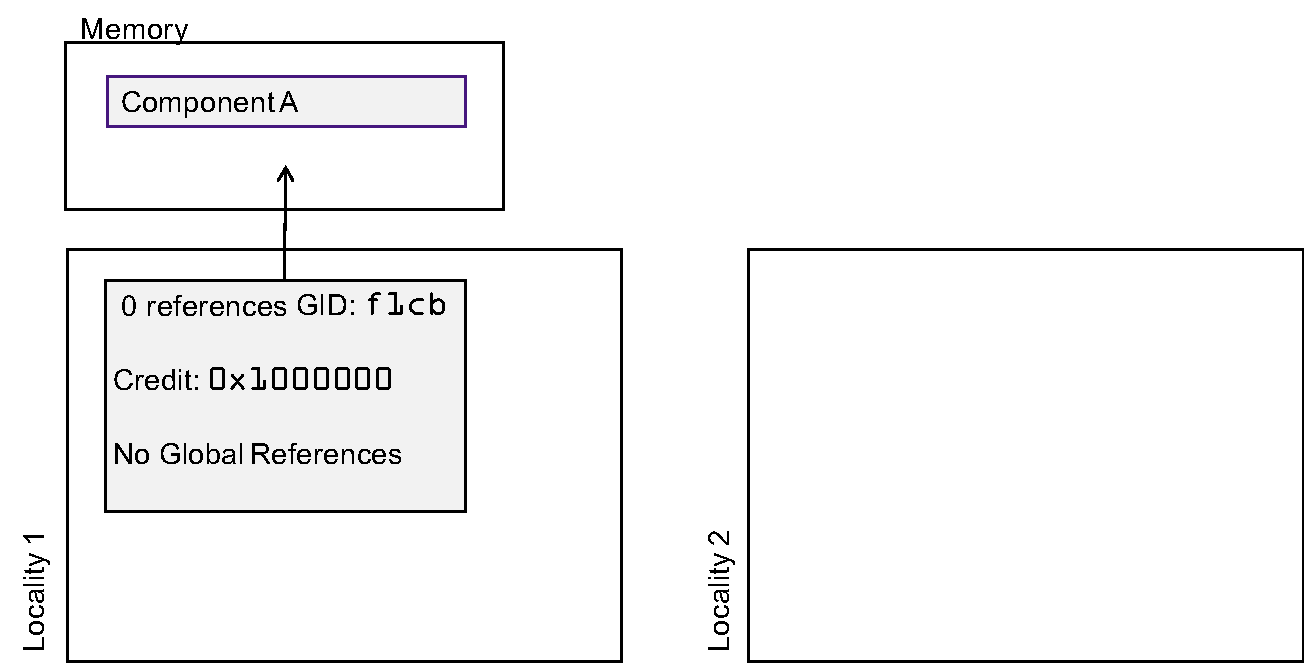
\includegraphics[width=\textwidth]{illustrations/reference_counting_1}
                \caption{An object is created. AGAS sets the object's credit to a large
                  number.}
                \label{fig:agas_credit_1}
            \end{subfigure}
            \vspace{2em}
            \hfill
            \begin{subfigure}[t]{0.49\textwidth}
                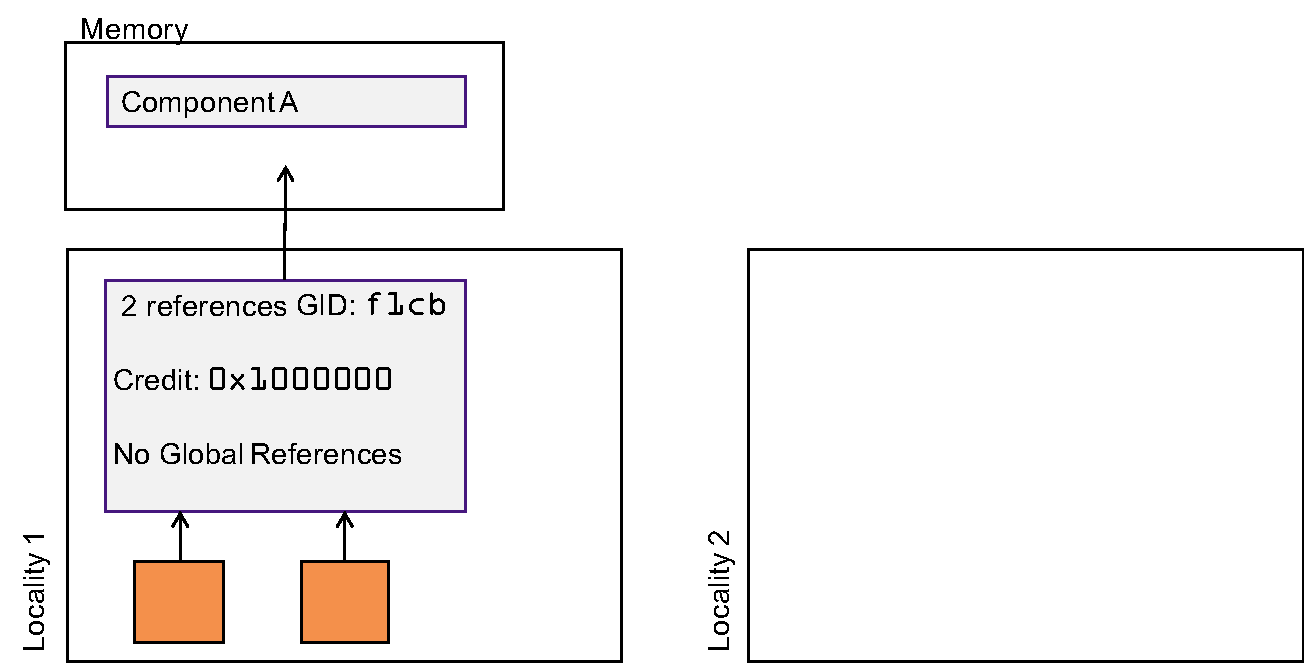
\includegraphics[width=\textwidth]{illustrations/reference_counting_2}
                \caption{A global object referenced by two local copies of the GID. Credit is not affected by local copies.}
                \label{fig:agas_credit_2}
            \end{subfigure}
            \begin{subfigure}[t]{0.49\textwidth}
                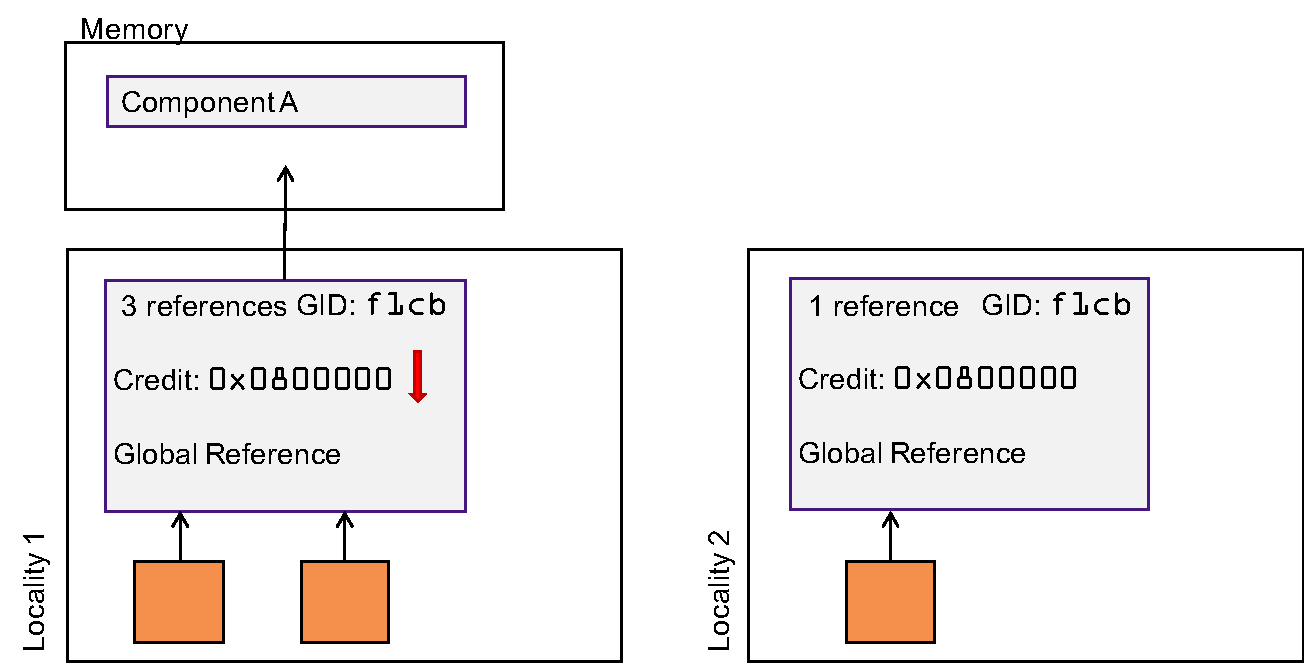
\includegraphics[width=\textwidth]{illustrations/reference_counting_3}
                \caption{When an object is referenced by another locality the object's
                  credit is split in half and a copy of the reference is kept at both
                  localities, and a flag is set on the original reference to
                  indicate that the object is referenced globally. When a copy
                  runs out of credit, it will ask the lender AGAS instance (the
                  locality where the reference is located) for more. If the
                  original reference itself does not have enough credit, the
                  AGAS instance responsible for that reference (where the
                  object resides) will grant it more credit.
                }
                \label{fig:agas_credit_3}
            \end{subfigure}
            \hfill
            \begin{subfigure}[t]{0.49\textwidth}
                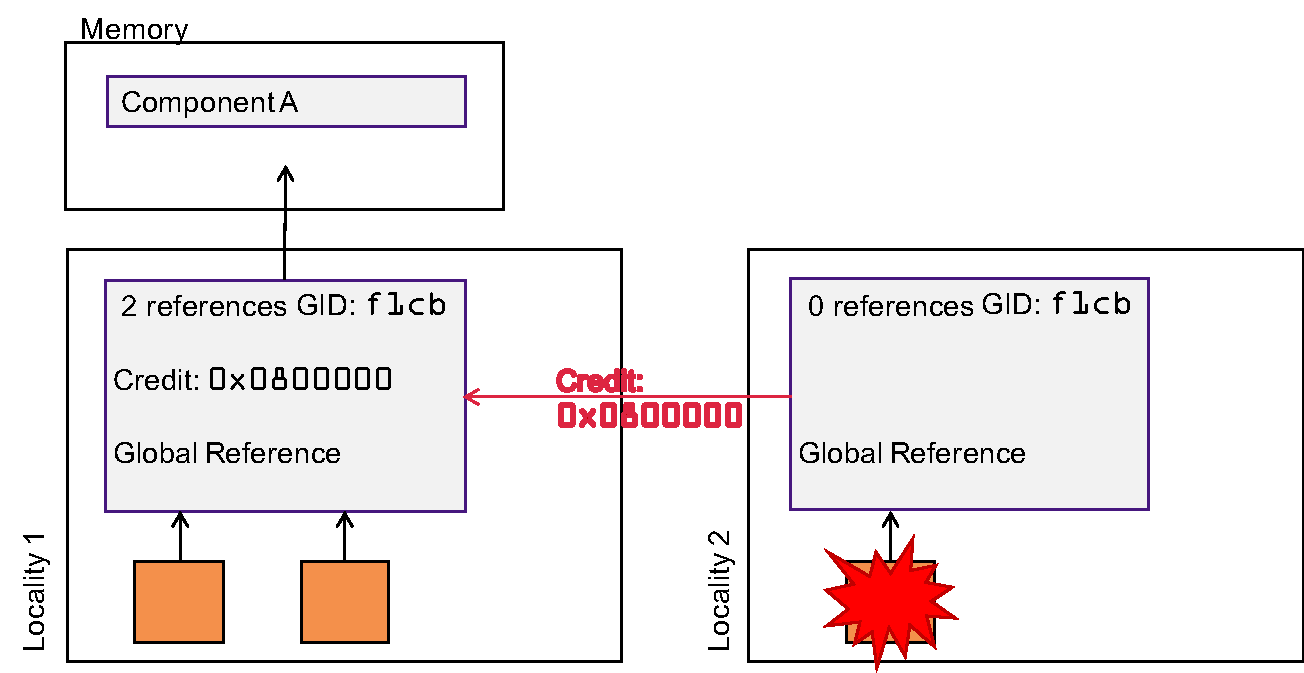
\includegraphics[width=\textwidth]{illustrations/reference_counting_4}
                \caption{When a reference goes out of scope AGAS returns all borrowed
                  credits to the original reference. If there are no local references and all credits have been
                  returned then AGAS can remove the object from memory during garbage
                  collection.}
                \label{fig:agas_credit_4}
            \end{subfigure}
            \caption{AGAS credit system tracks global references. When a global reference goes out of scope all of its credit is returned to the lender. When there are no local or global references the memory allocated by the object can be freed by the garbage collector.}
            \label{fig:agas_credit}
        \end{figure*}
\end{enumerate}

\begin{figure}[t]
    \centering
    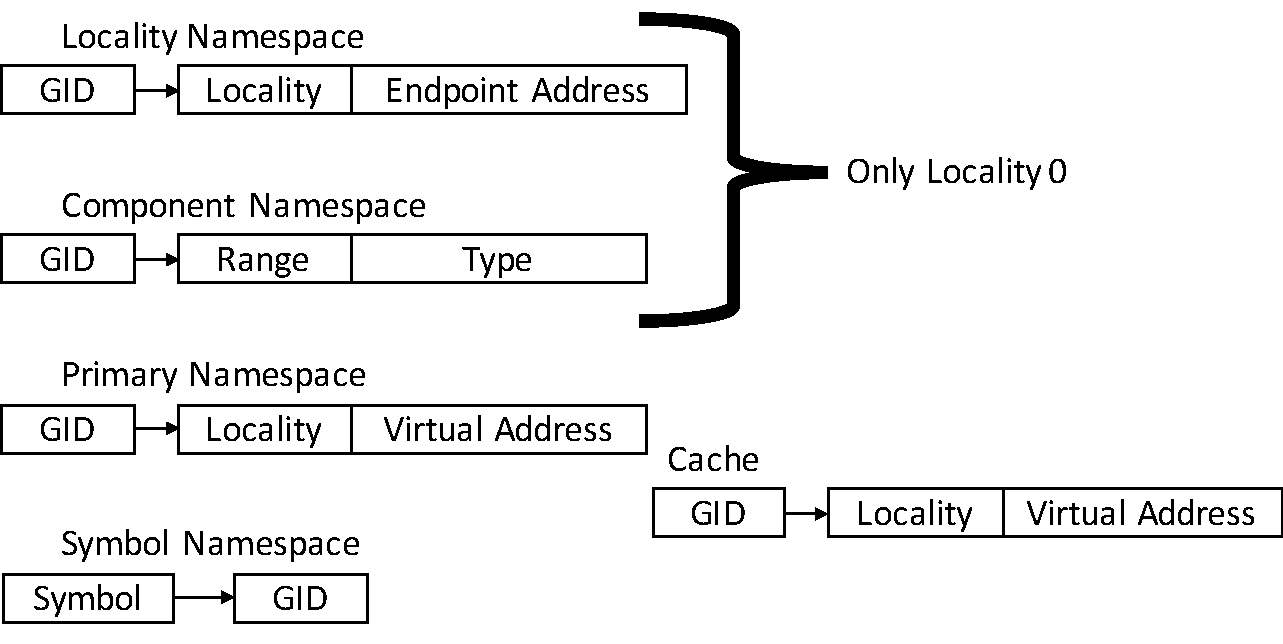
\includegraphics[width=.47\textwidth,height=\textheight,keepaspectratio]{illustrations/agas_intern}
    \caption{The four namespaces inside AGAS. Primary namespace on each AGAS instance contains GID to local address mappings. Locality namespace holds information about all AGAS instances. Component namespace tracks bulk memory allocations dedicated to types. Symbolic namespace contains mappings between GIDs and special strings that can be used for various purposes such as facilitating the collection of data about application execution.}
    \label{fig:agas_intern}
\end{figure}

Garbage collection at runtime requires execution of code that is otherwise not
present and consumes computing resources. Performing garbage collection
requires executing code that is the not the user's application. AGAS tries to
minimize garbage collection sweeps by performing it when the volume of garbage
reaches a certain threshold that can be specified by the users. It is also
possible to manually initiate it inside applications by developers.

\subsection{AGAS Performance Counters}
HPX is a runtime system that includes novel abstractions on top of ordinary
operating systems and hardware that are more difficult to benchmark using traditional
performance measuring tools such as hardware performance counters included in
Intel processors. HPX introduces a set of performance counters to let
developers monitor the performance of its subsystems, including AGAS, during
execution.

Similar to hardware performance counters, HPX performance counters\cite{grubel2015performance} are designed
to expose performance data on the underlying function calls. HPX has
performance counters that measure performance of AGAS subsystems. Each AGAS
performance counter either reports the number of invocations or the total
execution time of the selected operation.

\subsection{HPX bootstrap and teardown}
Before an HPX application can start executing, HPX has to initialize. This
process is called bootstrap and includes registering runtime services, data
types, performance counters, and symbols.
Similarly during teardown, after applications built with HPX complete, HPX removes all
objects, frees all allocated hardware resources and may perform additional
tasks such as collecting performance counter data when applicable.

In this research, we exclude data from the bootstrap and teardown phases since
they do not directly provide useful data on how AGAS might impact the
performance or scaling behavior during runtime.
